\documentclass[10pt]{beamer}
\usetheme{Antibes}
\usepackage[utf8]{inputenc} 
\usepackage[vietnam,english]{babel}
\usepackage{ragged2e}
\usepackage{graphicx}
\usepackage[dvips]{color}
% coding styles  %%%%%%%%%% font for code terminal
% \setbeamercovered{transparent}
\usepackage{listings}
\usepackage{xcolor}
\graphicspath{{./img/}}
\definecolor{codegreen}{rgb}{0,0.6,0}
\definecolor{codegray}{rgb}{0.5,0.5,0.5}
\definecolor{codepurple}{rgb}{0.58,0,0.82}
\definecolor{backcolour}{rgb}{0.95,0.95,0.92}
 
\lstdefinestyle{mystyle}{
    backgroundcolor=\color{backcolour},   
    commentstyle=\color{codegreen},
    keywordstyle=\color{magenta},
    numberstyle=\tiny\color{codegray},
    stringstyle=\color{codepurple},
    basicstyle=\ttfamily\footnotesize,
    breakatwhitespace=false,         
    breaklines=true,                 
    captionpos=b,                    
    keepspaces=true,                 
    numbers=left,                    
    numbersep=5pt,                  
    showspaces=false,                
    showstringspaces=false,
    showtabs=false,                  
    tabsize=2
}
 
\lstset{style=mystyle}
 
% end coding styles
\title{FTech Training}
\subtitle{Using Beamer}
\author{Luc Nguyen}
\institute{HUST}
\date{\today}
\usetheme{Boadilla}


\begin{document}
\begin{frame}
    \frametitle{\textbf{TEXT AUGMENTATION}}
    \Large{\textbf{OUTLINE}}
    \begin{enumerate}
        \item Idea
        \item Some techniques
        \begin{itemize}
            \item Thesaurus
            \item Word embeddings
            \item Back translation
            \item Contextualize word embeddings
            \item Text generation
            \item Random deletion
        \end{itemize}
        \item Some wellknown researches
        \begin{itemize}
            \item In English
            \item In Vietnamese
        \end{itemize}
        \item References %If you understand your data, you should tailor made augmentation approach it
    \end{enumerate}
\end{frame}
\begin{frame}
    \frametitle{\textbf{IDEA}}
    \begin{itemize}
        \item More data we have, better model, performance we can achieve.
        \item Training data is \textbf{NOT} unlimited.
        \item We need a techniques to generate more data.
    \end{itemize}
\end{frame}
\begin{frame}[fragile]
    \frametitle{\textbf{SOME TECHNIQUES}}
    \framesubtitle{\textbf{Thesaurus}}
    \begin{definition}[Thesaurus]
        Replace non-stop words or phrase with their synonyms.
    \end{definition}\pause
    \begin{definition}[Stop word]
        Words which are filtered out before processing of natural language data.
    \end{definition}\pause
    \begin{lstlisting}[language=Python, caption=Stop words in English ]
        import nltk
        from nltk.corpus import stopwords
        nltk.download('stopwords') # run only the first time
        print(set(stopwords.words('english')))
        # {'the', 'they', 'of', 'you', 'each', 'some', 'be', 'down', 's', 're', 'between', 'we', "mustn't", 'so', ... }
        print(len(set(stopwords.words('english'))))
        # 179
    \end{lstlisting}
\end{frame}
\begin{frame}
    \frametitle{\textbf{SOME TECHNIQUES}}
    \framesubtitle{\textbf{Thesaurus} - Automatic thesaurus generation}
    There are two main approaches:\pause
    \begin{itemize}
        \item Exploit word co-occurrence \pause
        \item Use a shallow grammatical analysis\pause
        \\ \vspace{15pt}
        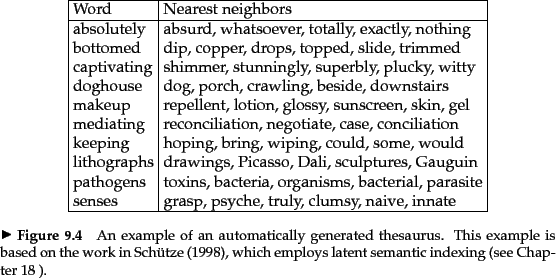
\includegraphics[scale = 0.45]{auto_thesaurus_generation.png}
    \end{itemize}
\end{frame}
\begin{frame}
    \frametitle{\textbf{SOME TECHNIQUES}}
    \framesubtitle{\textbf{Word embeddings}}
    \begin{definition}[Word embeddings]
        Represent a word by a high-dimensional vector where each dimension represents a value of a property
    \end{definition}\pause
    Example : \\
    \begin{center}
        \begin{math}
        \mbox{Guitar} = \begin{pmatrix} 0.12 \\ 0 \\ 0 \\ 0.74 \\ -0.89 \end{pmatrix}
        \mbox{Piano} = \begin{pmatrix} 0.67 \\ 0.8 \\ 0 \\ 0.22 \\ -0.80 \end{pmatrix} \pause
        \Longrightarrow\mbox{cos\_sim} = 0.6157
        \end{math} 
    \end{center}\\ \pause
    \begin{minipage}{0.4\textwidth}
        Some useful models for word embeddings: word2vec, GloVe, fastText 
    \end{minipage}
    \begin{minipage}{0.55\textwidth}
        \begin{center}
            \begin{figure}[]
                \centering
                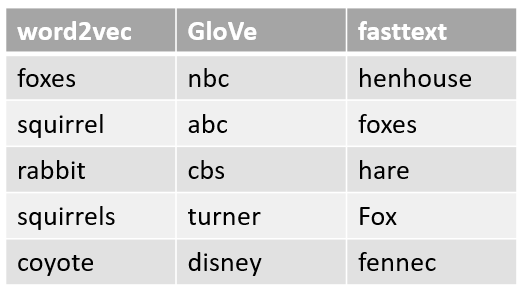
\includegraphics[scale=0.22]{word_embedding.png}
                \caption{Most similar words of \textit{fox} among classical word embeddings models}
                % \label{labb}
            \end{figure}
        \end{center}
    \end{minipage}
\end{frame}
\begin{frame}[fragile]
    \frametitle{\textbf{SOME TECHNIQUES}}
    \framesubtitle{\textbf{Word embeddings} - Gensim Word2Vec Model}
    \begin{itemize}
        \item Install \texttt{gensim, beautifulsoup4} library\\
        \texttt{pip install gensim beautifulsoup4}
        \begin{lstlisting}[language=Python, caption=Library importation]
        #import libraries
    from gensim.models import Word2Vec
    import bs4 as bs
    \end{lstlisting}\pause
    \item Other utility : \texttt{nltk.stem.PorterStemmer, nltk.stem.WordNetLemmatizer} \\
    Example : (programs, programming, programed, ...) = program 
\end{itemize}
\end{frame}
\iffalse
\begin{frame}[fragile]
    \frametitle{\textbf{SOME TECHNIQUES}}
    \framesubtitle{\textbf{Word embeddings} - Gensim Word2Vec Model}
    \begin{lstlisting}[language=Python, caption=Python example]
        # Preparing the dataset
    all_sentences = nltk.sent_tokenize(processed_article)
    all_words = [nltk.word_tokenize(sent) for sent in all_sentences]
        # Cleaing the text
    processed_article = article_text.lower()
    processed_article = re.sub('[^a-zA-Z]', ' ', processed_article)
    processed_article = re.sub(r'\s+', ' ', processed_article)
        # Removing Stop Words
    for i in range(len(all_words)):
        all_words[i] = [w for w in all_words[i]
                if w not in stopwords.words('english')]
    word2vec = Word2Vec(all_words, min_count=2)
    vocabulary = word2vec.wv.vocab
    print(word2vec.wv.most_similar('name'))
    \end{lstlisting}
\end{frame}
\fi
\begin{frame}
    \frametitle{\textbf{SOME TECHNIQUES}}
    \framesubtitle{\textbf{Back translation}}
    \begin{definition}[Back translation]
        Translate target language to source language and mixing both original
         source sentence and back-translated sentence to train a model
    \end{definition}\pause
    Example : \\
    English : I play soccer \newline
    Vietnamese :  $\Rightarrow$ Tôi chơi bóng đá \newline
    English : $\Rightarrow$ I play football
\end{frame}
\begin{frame}
    \frametitle{\textbf{SOME TECHNIQUES}}
    \framesubtitle{\textbf{Text generation}}
    \begin{definition}[Text generation]
        Generate text with the goal of appearing indistinguishable to human-written text.
    \end{definition}\pause
    Some useful libraries/techniques : 
    \begin{itemize}
        \item LSTM Recurrent Neural Networks in Python with Keras
        \item N-gram, RNNs, GRUs, LSTMs, seq2seq(Conditional Language Model)
    \end{itemize}\pause
    Example :  \\
    When we type : \textsf{as soon as} \\
    \pause
    Google suggest : \textsf{as soon as\left|  {\color[named]{gray} possible}}
\end{frame} 
\begin{frame}
    \frametitle{\textbf{SOME TECHNIQUES}}
    \framesubtitle{\textbf{Random deletion}}
    \begin{definition}
        Randomly remove one (or many) word(s) from a sentence to create a now sentence.
    \end{definition}\pause
    Example : \\
        Original:     \textrm{The quick brown fox jumps over the lazy dog}\\
        Augmented Text:    \textrm{The fox jumps over the lazy dog}
\end{frame}
\begin{frame}
    \frametitle{\textbf{SOME WELLKNOWN RESEARCHES}}
    \begin{itemize}
        \item In English
        \begin{itemize}
            \item Gmail suggestion while composing.
            \item Google BERT
            \item Facebook RoBERTa.
            \item Amazon sagemaker.
        \end{itemize}\pause
        \item In Vietnamese
        \begin{itemize}
            \item Vietnam Language and Speech Processing (https://vlsp.hpda.vn/)
        \end{itemize}
    \end{itemize}
\end{frame}
\begin{frame}
    \frametitle{\textbf{REFERENCES}}
    \begin{enumerate}
        \item https://towardsdatascience.com/data-augmentation-library-for-text-9661736b13ff 
        \item https://towardsdatascience.com/data-augmentation-in-nlp-2801a34dfc28 
        \item https://www.kilgarriff.co.uk/Publications/2003-K-Beijing-thes4NLP.pdf 
        \item https://vlsp.hpda.vn/demo 
        \item https://nlp.stanford.edu/IR-book/html/htmledition/automatic-thesaurus-generation-1.html 
        \item https://stackabuse.com/implementing-word2vec-with-gensim-library-in-python/ 
        \item https://towardsdatascience.com/exploring-wild-west-of-natural-language-generation-from-n-gram-and-rnns-to-seq2seq-2e816edd89c6 
        \item https://docs.aws.amazon.com/sagemaker/latest/dg/whatis.html 
    \end{enumerate}
\end{frame}
\begin{frame}
	\frametitle{\textbf{LINEAR REGRESSION}}
	\framesubtitle{Idea}
	\begin{itemize}
		\item Linear regression is a linear approach to modeling the relationship between a scalar response and one or more explanatory variables.
		\item Type of linear regression : 
		\begin{itemize}
			\item Simple linear regression : $ \hat{y} = xw + b $
			 \\ where $\hat{y}, x, w, b$ is a scalar variable.
			\item Multivariate linear regression : $ \hat{y} = xw + b = \bar{x}w$
			 \\ where $w, x$ are vectors, $\hat{y}, b$ is a scalar number.
		\end{itemize}
    \end{itemize}
\end{frame}
\end{document}